\subsection{Baseline predictions}

We began by establishing a baseline model for bass guitar tablature generation.
Initially, we utilized a pre-trained checkpoint from the DadaGP paper \cite{sarmento_dadagp_2021} without additional training.

To generate bass-specific outputs, we experimented with various prompts.
First, we provided a single bass guitar note as the initial token, however the model quickly incorporated tokens from other instruments.
This is an issue documented in the GuitarCTRL paper\cite{sarmento_gtr-ctrl_2023} where they used a metric called the UIP score (Unpromped Instrument Presence) to evaluate the model's ability to generate a specific combinations of instruments.
To constrain the output to bass tokens, we modified the logits of non-bass instruments by setting them to $-\infty$.

% FIGURE REPETITIVE GENERATION
\begin{figure}[!ht]
    \centering
    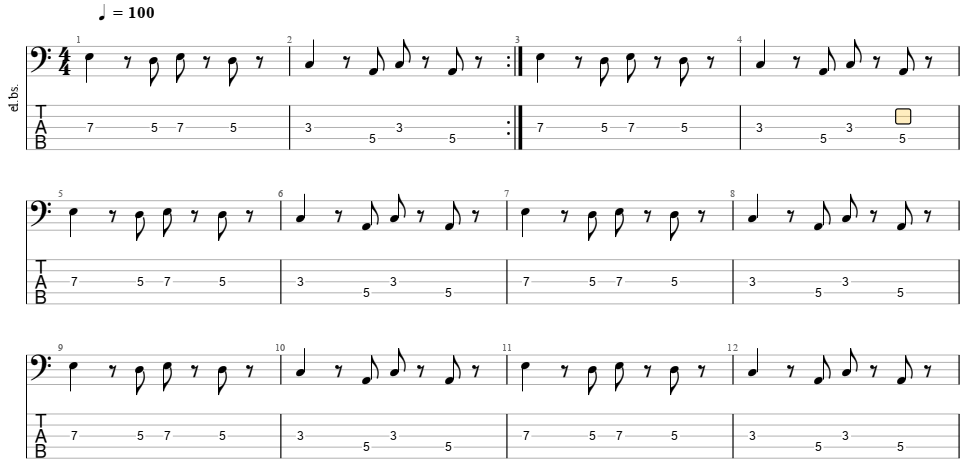
\includegraphics[width=.75\linewidth]{../images-figures/generated_bass_baseline.png}
    \caption{Example of a bass generation from the baseline model}
    \label{fig:repetitive_generation}
\end{figure}

An example of a bass tablature generated this way is shown in Figure~\ref{fig:repetitive_generation}.
While this forced the model to generate only bass tokens, the output quality was poor, featuring repetitive phrases, harmonically incorrect notes, or complete aberrations.
This was expected, as the model was not trained explicitly for bass only generation. 
Unfortunately, we cannot provide a quantitative evaluation of the generated tablatures, as we have not yet defined an evaluation metric.

\subsection{BiLSTM - Transformer model}

This section present the results we get using a model adapted from the work of Makris et al. \cite{makris_conditional_2022}.
Our data was adapted to fit the model's input requirements and the model was also slightly modified to fit our task.

% FIGURE MAKRIS ET AL. MODEL
\begin{figure}[!ht]
    \centering
    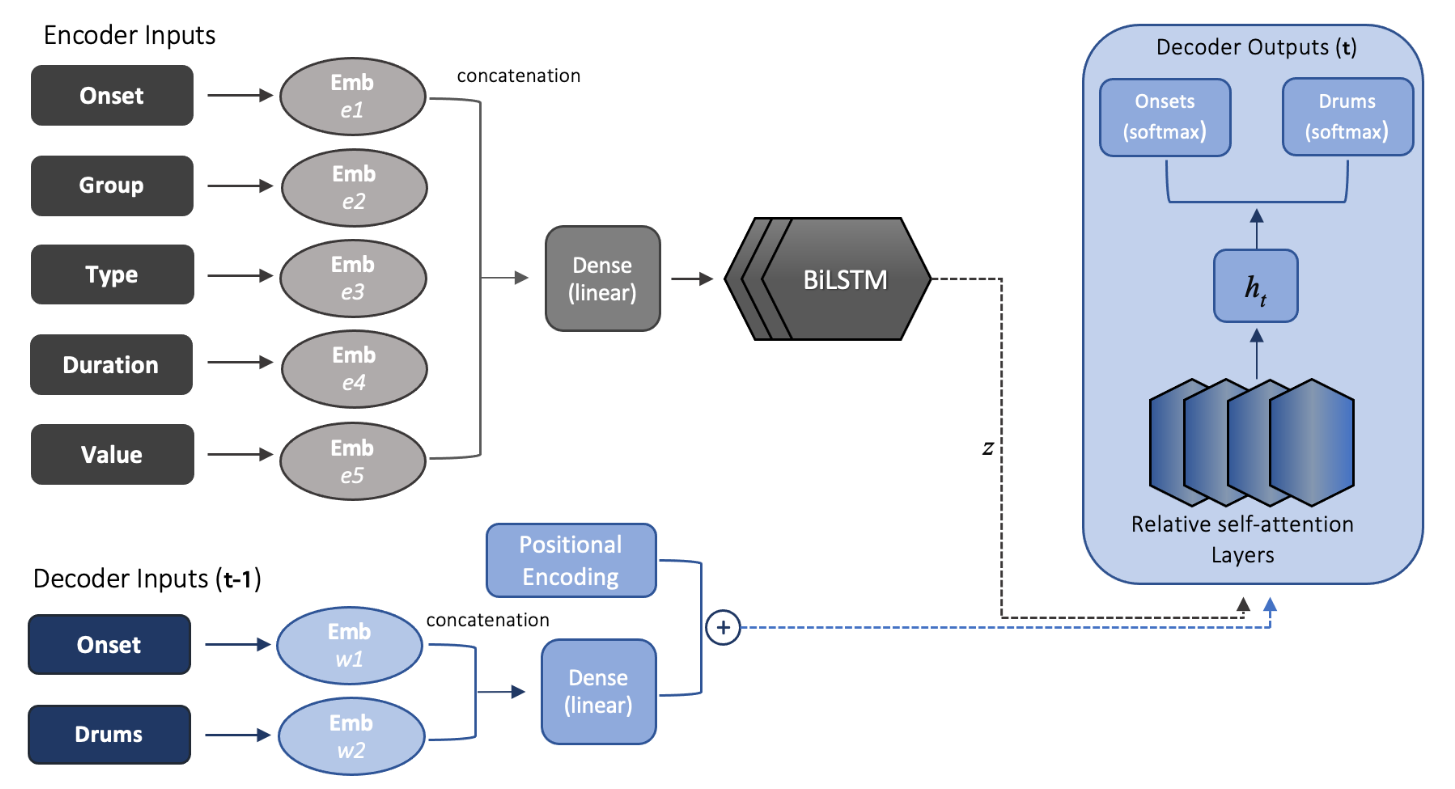
\includegraphics[width=.75\linewidth]{../images-figures/makris_model.png}
    \caption{Makris et al. model architecture, taken from their paper \cite{makris_conditional_2022}}
    \label{fig:makris_model}
\end{figure}

The figure~\ref{fig:makris_model} shows the architecture of the model proposed by Makris et al.
We have presented the compound representation in the state of the art.
This representation concatenates all the parameters necessary to describe a note in a single vector (onset, duration, pitch etc.).

% FIGURE MAKRIS ET AL. MODEL ADAPTED TO OUR TASK
\begin{figure}[!ht]
    \centering
    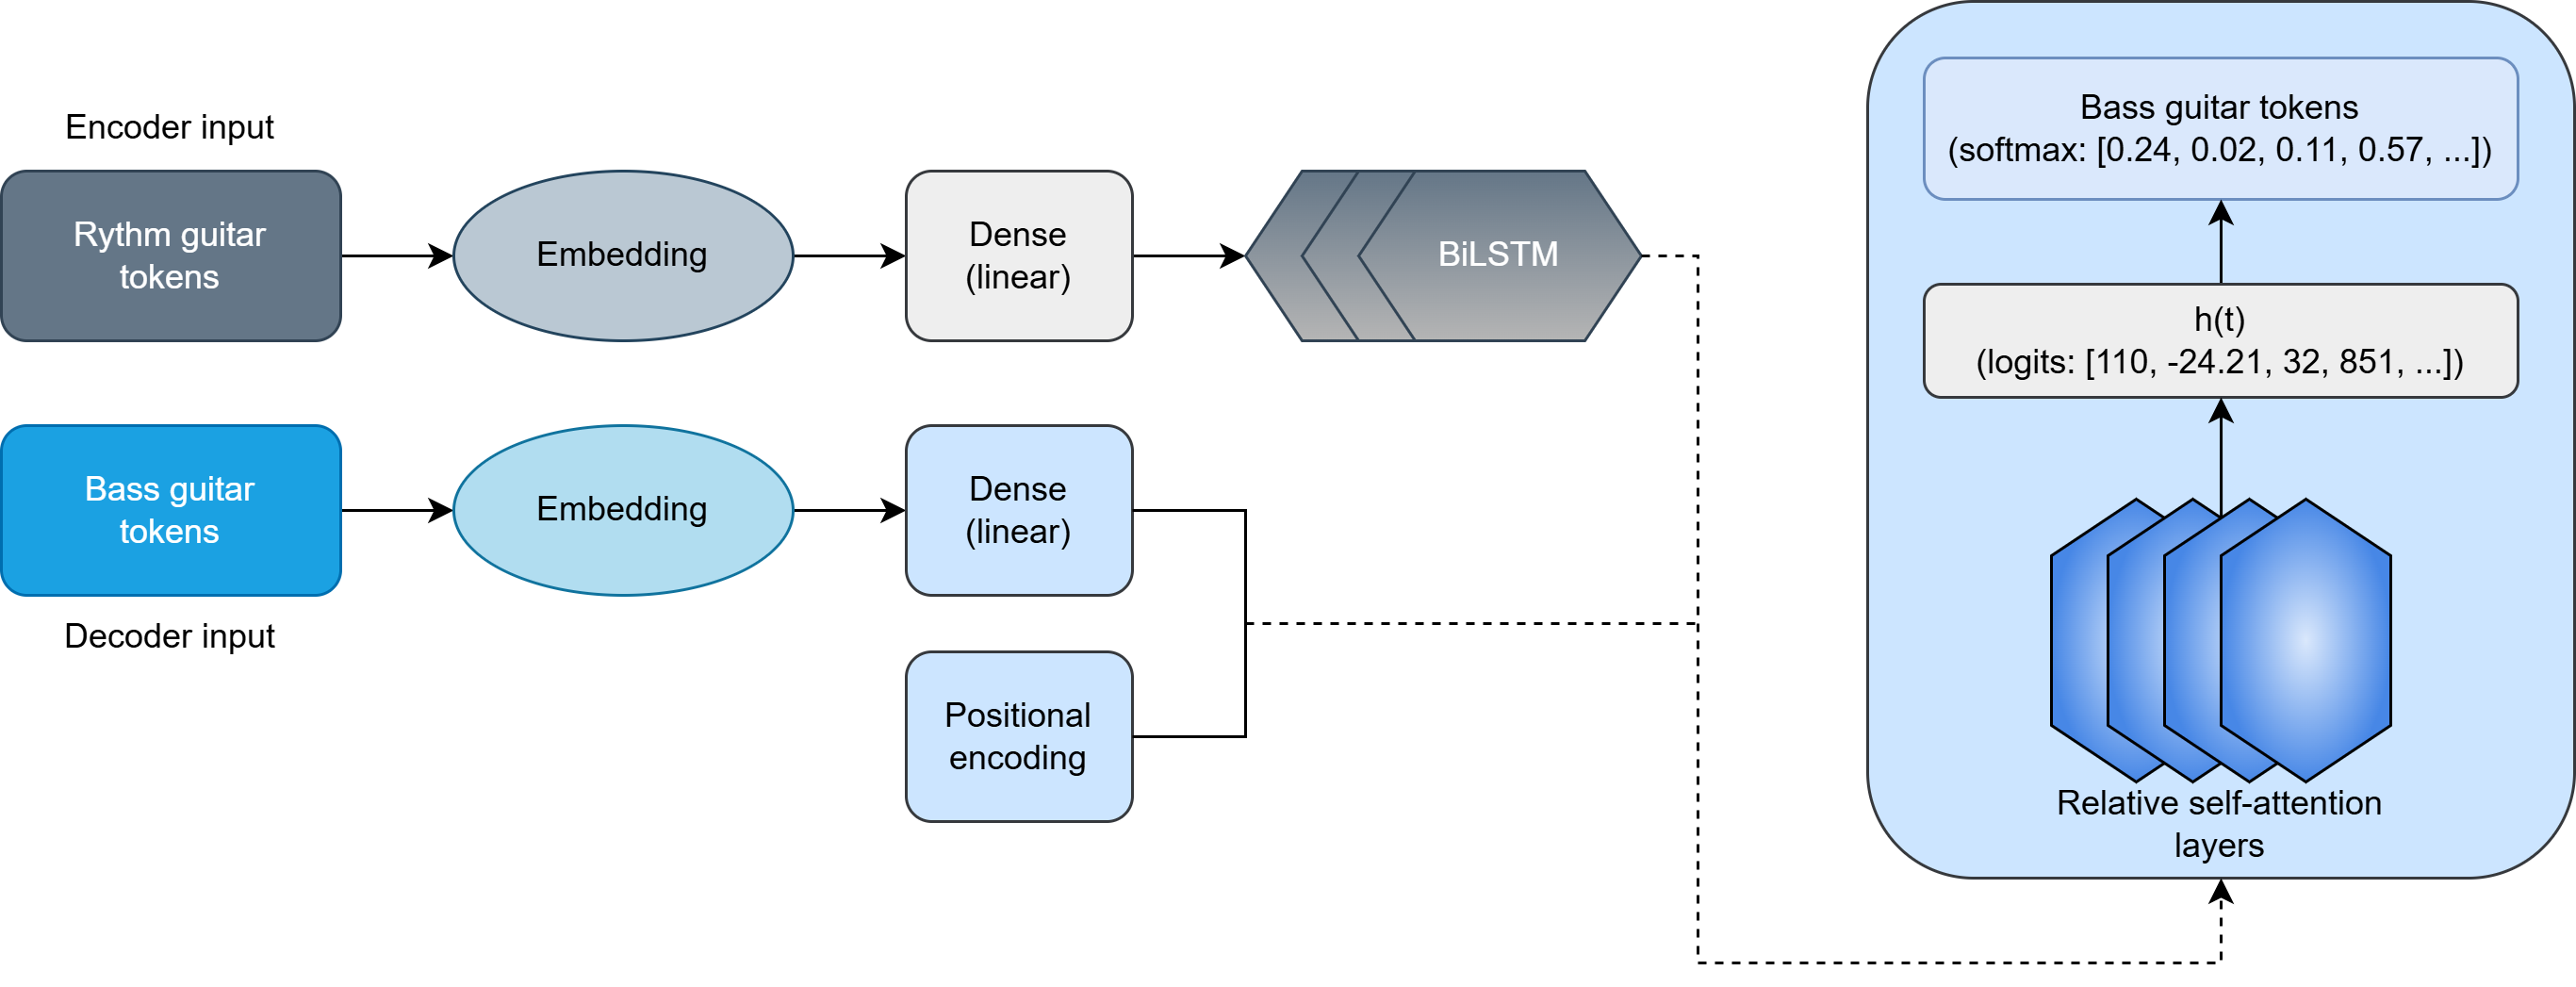
\includegraphics[width=.75\linewidth]{../images-figures/model_adapted.png}
    \caption{Makris et al. model adapted to our task}
    \label{fig:makris_model_adapted}
\end{figure}

Figure \ref{fig:makris_model_adapted} shows the model adapted to our task.
In our case, we have chosen to use DadaGP tokenization which is a different representation.
On the encoder side, the five embeddings concatenated in Makris et al. are replaced by a single embedding in our case.
On the decoder side, their input had a special shape because drums notes need much less parameters than other instruments.
They are fully described by their onset and a value indicating the drum type.
This compound representation is also replaced by a single embedding in our case.

The embeddings are then passed through a dense layer. The encoder input (rythmic guitar) is passed through a BiLSTM layer.
Positional encodings are added to the decoder input and the output of the BiLSTM layer.
All these elements are then passed through a transformer layer with self-attention mechanism
that outputs an array of vocabulary size with the probability of each token.

\subsection{Training and inference}

The model was trained on 11 020 extract from songs in the DadaGP dataset.
These extracts are the first 16 measures of the song, and contain sequences of at most 800 tokens and at least 50 tokens.
Thresholds were set to avoid training on sequences that are either too long or that does not contain rythmic guitar or bass.

% FIGURE DISTRIBUTION OF SEQUENCE LENGTHS
\begin{figure}[!ht]
    \centering
    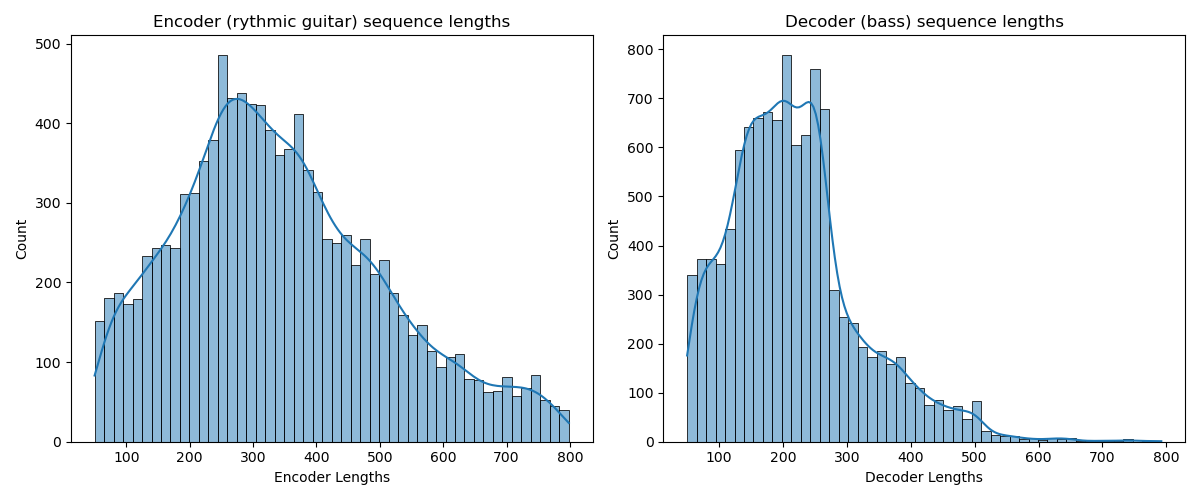
\includegraphics[width=.75\linewidth]{../images-figures/sequence_lengths_16_800_50.png}
    \caption{Distribution of sequence lengths in the training dataset}
    \label{fig:sequence_length_distribution}
\end{figure}

Figure \ref{fig:sequence_length_distribution} shows the distribution of sequence lengths in the training dataset.
The majority of the sequences are between 200 and 400 tokens long for the rythmic guitar and between 100 and 300 tokens long for the bass.

Training was done on GPU with 200 epochs and a batch size of 32.
However the training stopped at epoch 29 because the validation loss did not decrease anymore for 5 epochs.
We reached 0.90 accuracy on the validation set with 0.42 loss.